%! TEX root = 'main.tex'

\section{Background}
\label{sec:ktoctou-background}


TOCTOU is a vulnerability class caused by changes in a system between checking a condition and using that check results. Typically, a variable or system state changes after it passes the sanity check. It is a classic vulnerability, mostly amount file system APIs. Many previous research works have addressed it~\cite{dean2004fixing}~\cite{borisov2005fixing}. Before introducing the relatively new kernel-level TOCTOU, we first briefly describe the classic TOCTOU as shown in~\autoref{fig:toctou}.


\begin{figure}[th]
	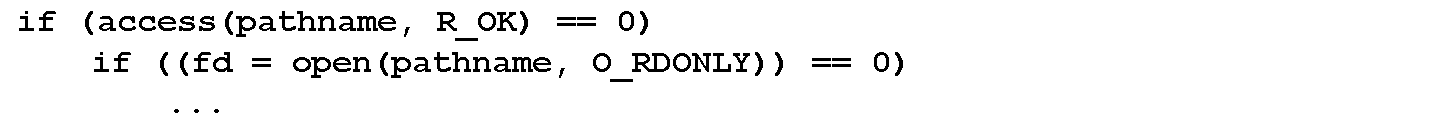
\includegraphics[width=0.47\textwidth]{figures/toctou}
	\centering
	\caption{The gap between access() and open() leaves the attack time window for the attacker to make changes in the file system.}
	\label{fig:toctou}
\end{figure}

%\begin{lstlisting}[basicstyle=\small,style=redkeyword]
%\begin{lstlisting}[style=code]
%if (access(pathname, R\_OK) == 0)
%    if ((fd = open(pathname, O\_RDONLY)) == 0) ...
%\end{lstlisting}



Assume this code piece belongs to a setuid program. It first validates that the ``pathname'' is readable, and if so, open the file for reading. However, the attacker can change the file system between the two system calls to trick the setuid program into opening a file that it should not.

%Essentially, TOCTOU vulnerability occurs between security boundaries. The less privileged sector deceives the privileged sector to do unexpected actions. The non-atomic or repeated operation on the same variable is the root cause.


\subsection{Kernel-level TOCTOU Vulnerability}


TOCTOU also happens in the operating system kernel, inside system calls. For the rest of the paper, we name it kernel-level TOCTOU. An operating system provides services such as \texttt{program execution}, \texttt{I/O operation}, \texttt{file system} to the programs on a service-client basis. When requesting a system service, the programs provide parameters, and how to invalidate them, keep them consistent during the system call is the kernel's responsibility. However, due to various reasons, the kernel may not fully decouple with the user-mode components. Therefore, directly accessing user-mode variables from the kernel is not uncommon to some operating systems, especially Windows.

When the kernel repeatedly reads the same user-mode address, so-called double fetches, this type of behavior may lead to severe issues, typically local privilege escalation vulnerability. The malicious program first has a benign variable in userspace, then uses another thread to change the variable to bypass the parameter sanity check or introduce errors such as a buffer overflow in-between the kernel's two fetches. The time window between the two kernel fetches may be as short as several instructions,  but with careful design, the race condition created between the kernel and the user program makes it feasible, especially on a multi-processor system.



The correct way of handling user-mode parameters is to ``capture'' (copy) them first, then use the kernel copy for the rest of the system call. It is better to put such standard code into gateway functions for the kernel and drivers, such as those used in the Linux kernel, \texttt{copy\_to\_user()}, and \texttt{copy\_from\_user()}.

However, due to mistakenly repeated operations on user parameters, the kernel-level TOCTOU still widely exists among operating systems already taking the aforementioned method. ~\autoref{table:cves} lists a portion of recent kernel-level TOCTOU vulnerabilities.

\begin{center}
\begin{table}[ht]
%\singlespacing
%\scalebox{0.8}{
\small
\caption{Recent vulnerabilities categorized as race condition or time-of-check-to-time-of-use in the CVE database.}
\label{table:cves}
\centering
	\begin{tabular}{@{}>{\raggedright\arraybackslash}m{2.35cm}@{}|
			@{}>{\centering\arraybackslash}m{1.35cm}@{}|
			@{}>{\centering\arraybackslash}m{2.35cm}@{}|
			@{}>{\centering\arraybackslash}m{1.25cm}@{} } 
\hline
CVE-ID & Affected System & CVE-ID & Affected System \\ %[0.5ex]
\hline
CVE-2008-2252  & Windows & CVE-2016-5728 & Linux \\
CVE-2013-1280  & Windows & CVE-2016-6130 & Linux \\
CVE-2018-7249  & Windows & CVE-2020-9796 & macOS \\ 
CVE-2020-9839  & macOS   & CVE-2020-9990 & macOS \\
CVE-2016-10439 & Android & CVE-2016-7624 & macOS \\
CVE-2016-10383 & Android & CVE-2017-7115 & iOS \\

CVE-2020-5967  & Nvidia  & CVE-2020-8680 & Intel \\
\hline

\end{tabular}
\end{table}
\end{center}



%Notice that large part of the vulnerabilities of this table (from CVE-2013-1248 to CVE-2013-1280) are fixed in one Windows patch MS13-016, they are found by Gynvael Coldwind and Mateusz Jurczyk with Google Security Team. Due to the nature of kernel TOCTOU, it's difficult to exposure them in normal ways of testing or daily usage, until certain pattern and methods are found~\cite{jurczyk2013identifying}.  

%\begin{comment}
%\begin{figure}[th]
%  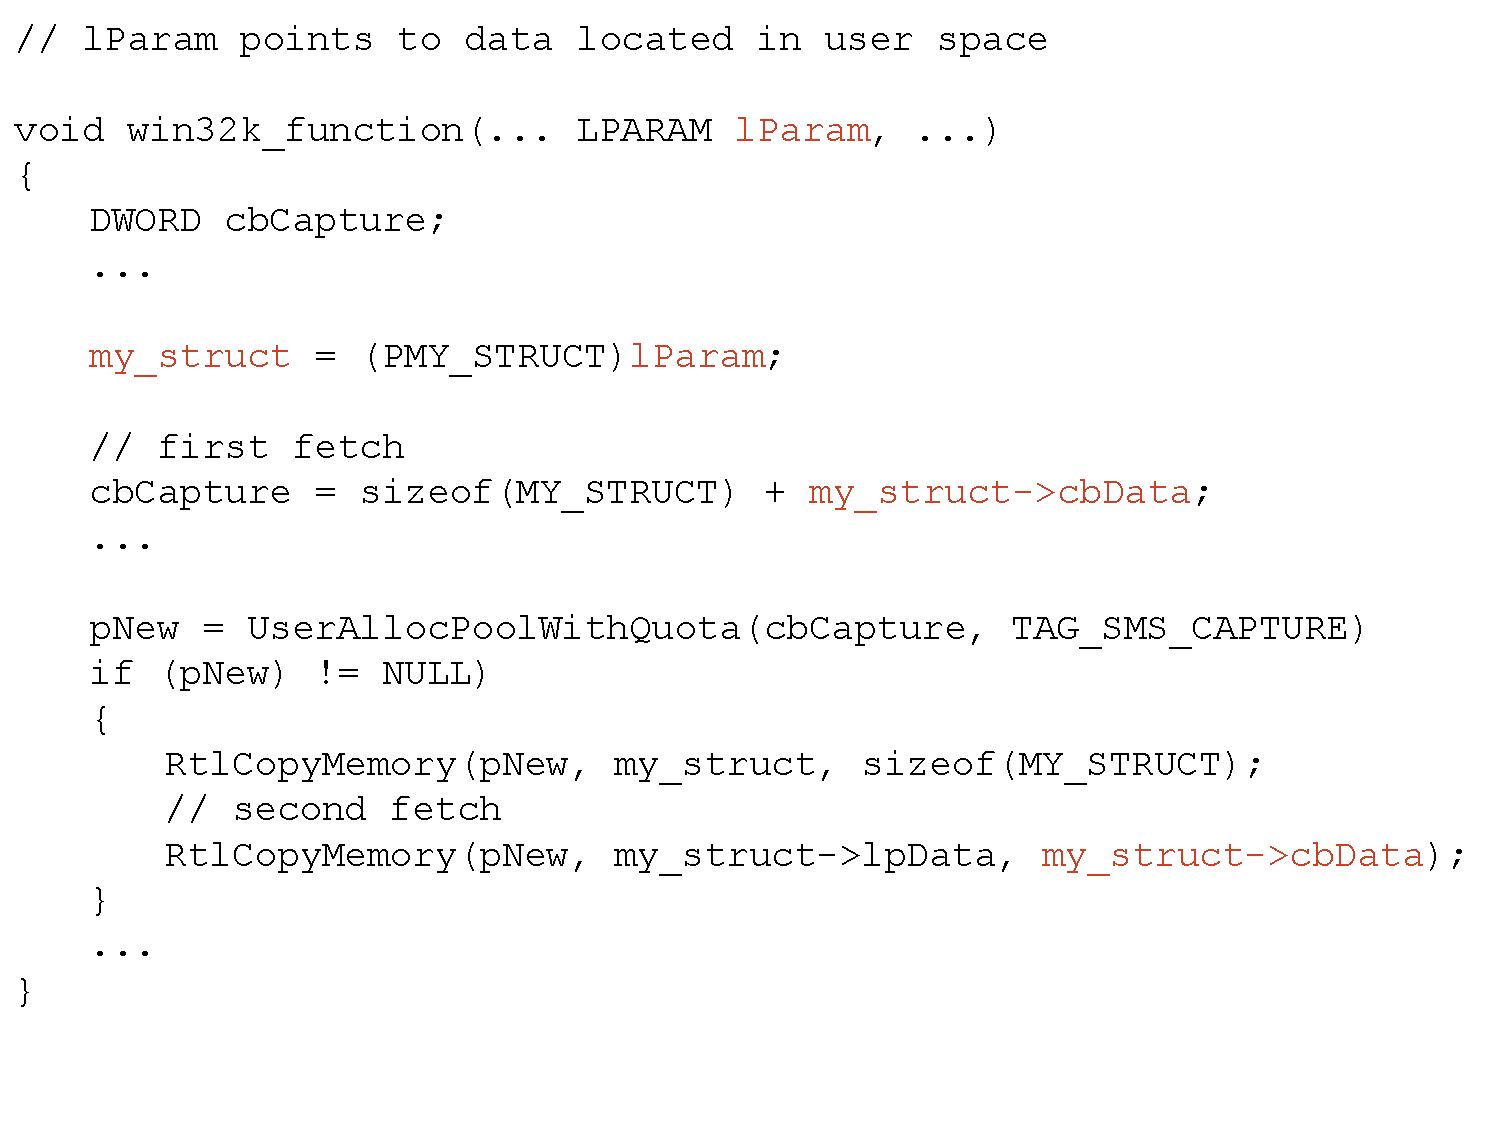
\includegraphics[width=0.47\textwidth]{toctouexample}
%  \centering
%  \caption{Sample code which has TOCTOU vulnerability. Data with in user space is referenced twice during a kernel pool allocation and data copying. ~\cite{jurczyk2013identifying}~\cite{ms08061}}
%  \label{fig:toctouexample}
%\end{figure}
%\end{comment}


%lst:vulnerablecode
%\begin{lstlisting}[style=code,caption={An snippet of Windows device driver code that mimic the vulnerability that fixed in ms08-061. The vulnerable user-mode variable is marked in red.}\label{lst:vulnerablecode}, captionpos=b]
%// lParam points to data located in user space
%void win32k_function(... LPARAM @lParam@, ...) 
%{
%    DWORD cbCapture;
%    ...
%    @my_struct@ = (PMY_STRUCT)@lParam@;
%
%    // first fetch
%    cbCapture = sizeof(MY_STRUCT) + @my_struct->cbData@;  
%    ...
%    pNew = UserAllocPoolWithQuota(cbCapture, TAG_SMS_CAPTURE)
%    if (pNew != NULL) 
%    {
%        RtlCopyMemory(pNew, my_struct, sizeof(MY_STRUCT);
%        // second fetch
%        RtlCopyMemory(pNew, my_struct->lpData, @my_struct->cbData@);   
%    }
%    ...
%}
%
%\end{lstlisting}


\begin{figure}[th]
	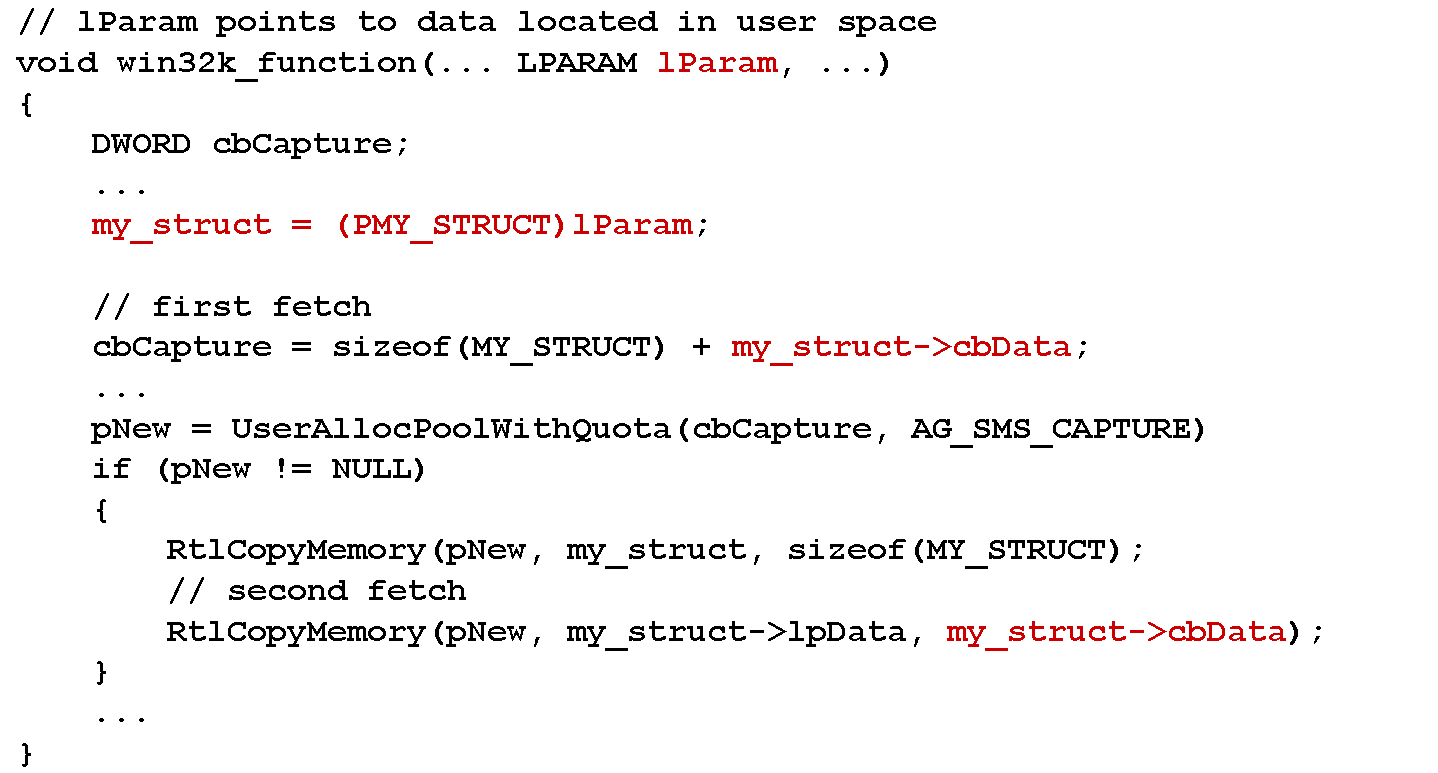
\includegraphics[width=0.47\textwidth]{figures/code08061}
	\centering
	\caption{Pseudocode of the vulnerability fixed in ms08-061. The vulnerable variable is in red. The kernel reads it twice, and it may get a different value for the buffer allocation and the subsequent buffer copying. It is common to see such a coding style. However, it is vulnerable because the two reads cross the privilege boundary.}
	\label{fig:code08061}
\end{figure}



~\autoref{fig:code08061} shows a piece of code from Windows Win32k module~\cite{jurczyk2013identifying}~\cite{ms08061}. This pseudo-code mimics a kernel-level TOCTOU vulnerability that has been identified and patched in ms08-061. It is part of the Win32k system call, and the code in red indicates the trace of the vulnerable code and data.  The user program passes \texttt{lParam} to \texttt{win32k\_function()} through upper layer API.  The first fetch occurs when summing up \texttt{cbCapture} with \texttt{my\_struct->cbData}, a data field offsetted from the address provided by \texttt{lParam}. The kernel allocates a buffer based on the data. However, shortly after, the kernel unnecessarily fetches this data again and uses it to copy data into the new buffer. As mentioned earlier, if the  \texttt{my\_struct->cbData} changes between the two fetches, especially when the last fetch gets a larger value, it will create a kernel heap buffer overflow. 

The attack time window is small, but enough. Even on a single processor system, the attack is feasible. For example, try to introduce a thread context switch between the two fetches. Because, for a local privilege escalation vulnerability like this, the attacker can invoke such a system call as many times as he needs. On a multi-processor system, the attacker usually creates another thread to race with the kernel, aiming at enlarging the data during the time window. As shown in~\autoref{fig:toctouasm}, the attacking thread 1 keeps flipping one higher bit of the variable. The attack succeeds by chance. If the latter value is smaller or equal to the former, the system will continue without error. If otherwise, the heap buffer overflow occurs.




\begin{figure}[ht]
  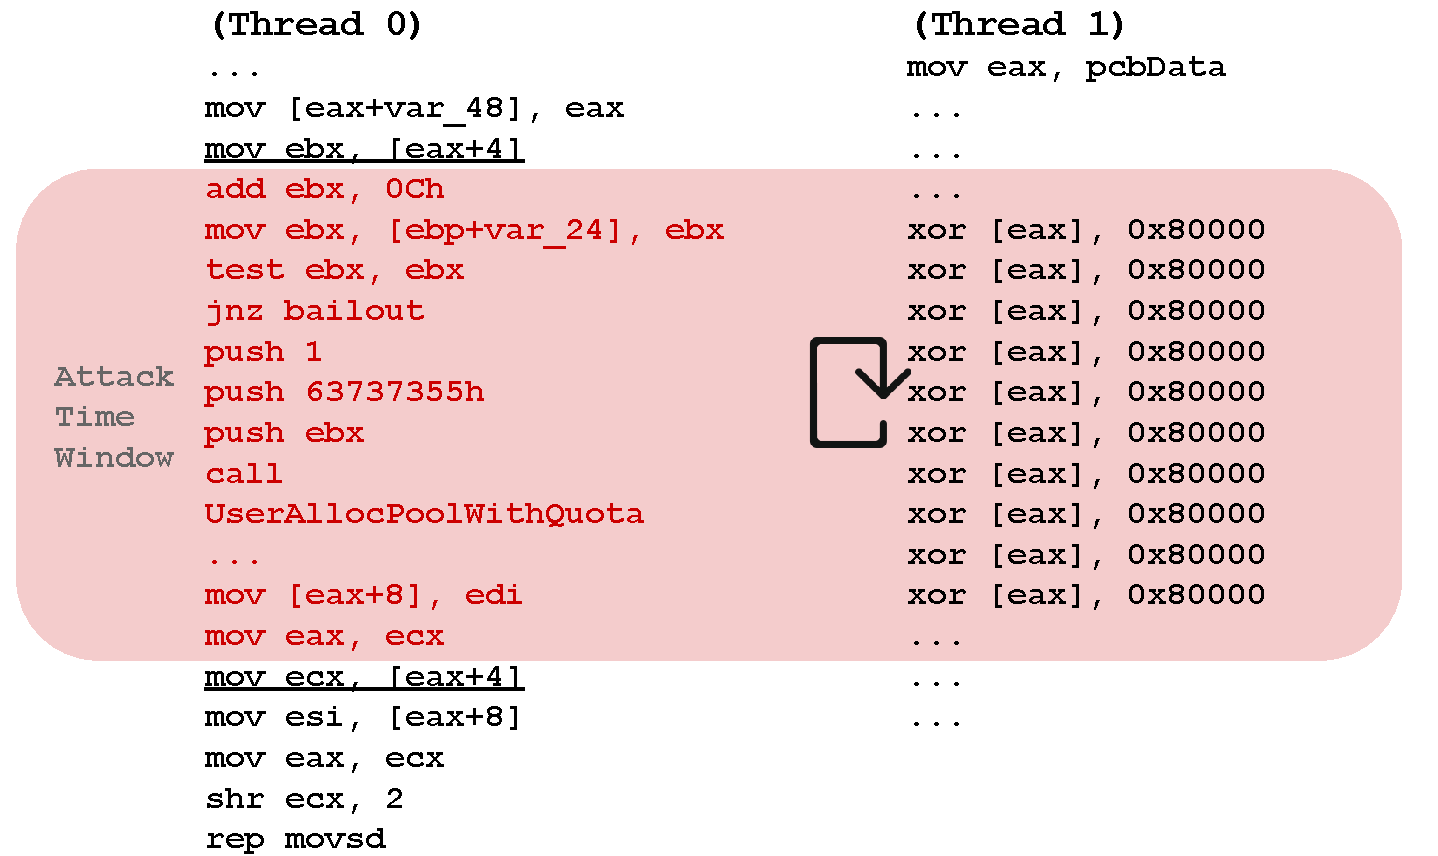
\includegraphics[width=0.47\textwidth]{figures/toctouasm3}
  \centering
  \caption{Thread 0 runs the vulnerable system call in the kernel-mode. The attacker can repeatedly call it to open the attack time window multiple times. Simultaneously, the other user-mode thread created by the attacker tries to flip the user-mode variable in-between the time window. So that the kernel code, two times, get the value differently.}
  \label{fig:toctouasm}
\end{figure}


%Once this step is accomplished, the problem becomes how to exploit it a classic heap buffer overflow. So you can see that kernel TOCTOU itself may not seems to be harmful, but it could lead to something serious. 

\subsection{Supervisor Mode Access Prevention (SMAP)}

%Kernel TOCTOU only needs accurate timing and memory writing, it's too plain to trigger any security mechanism so far. Existed monitoring methods are either too slow or too narrow, more details in~\autoref{sec:ktoctou-relatedwork}. We found a Intel CPU feature, Supervisor Mode Access Prevention (SMAP) is suitable for this task. 

%It's a security feature since Broadwell microarchitecture. It prevents operating system kernel directly accessing user-mode memory, which raises an exception. The intension is to stop transferring malicious payload from user space to kernel space.

%SMAP is enabled when the SMAP bit(21) in the CR4 is set. SMAP can be temporarily disabled for explicit memory accesses by setting the EFLAGS.AC (Alignment Check) flag. Because kennel does need to legally get data from user space, two more new instructions STAC (set AC flag) and CLAC (clear AC flag) are provided to accomplish that. The idea is that the kernel should be aware of when it's doing so. 

%For example, Linux kernel support for SMAP since version 3.7. All the accesses to user mode memory must go through two gateway functions \texttt{copy\_to\_user()} and \texttt{copy\_from\_user()}, where SMAP is temporarily disabled.

%However, Windows doesn't support SMAP yet. Different from Linux's approach, each of Windows syscalls tends to ``probe'' and ``capture'' user-mode data itself. Probing usually done by function ProbeForRead()~\cite{probeforread} and ProbeForWrite() to check the validity of the buffers, it also checks if a user mode buffer actually resides in the user space by simply compare its address to a pre-defined value. Since some modules such as win32k.sys are highly coupled with user-mode components, it will cost huge engineering effort to change the way it retrieve user-mode data.

%In Linux, even though \texttt{copy\_*\_user()} is mandated~\cite{corbet2012linuxsmap}, it still suffers from TOCTOU vulnerability such as mistake of using function \texttt{copy\_from\_user()} twice for the same variable~\cite{double-fetch-linux}. 



Monitoring the kernel's userspace behavior is essential to \name. Due to x86 protected mode characteristics, there is no mechanism available for a broad range of monitoring memory modifications. Techniques such as leveraging hardware watchpoints or transactional memory are fittable for fuzzing such vulnerabilities in a small memory range. However, none of them is realistic for run-time system protection. We discuss more details in~\autoref{sec:ktoctou-experiment} and~\autoref{sec:ktoctou-relatedwork}.

Fortunately, we notice an Intel CPU feature so-called \texttt{Supervisor Mode Access Prevention (SMAP)}~\cite{corbet2012supervisorsmap}~\cite{mulnix2016intel} accurately serves the purpose.
\texttt{SMAP} is a feature since the Intel Broadwell microarchitecture prevents the kernel from freely accessing userspace so that such access will raise an exception. It complements \texttt{Supervisor Mode Execution Prevention (SMEP)}~\cite{fischer2011supervisor} that introduced earlier. \texttt{SMEP} can be used to prevent the kernel from unintentionally executing user-mode code. \texttt{SMAP} extends this protection to reads and writes. It makes it harder for a malicious program to deceive the kernel into using code or data from the userspace.

\texttt{SMAP} is enabled when \texttt{CR4.SMAP} sets to 1. SMAP can be temporarily disabled for direct memory accesses by setting the \texttt{EFLAGS.AC} flag, and the \texttt{stac} and \texttt{clac} instructions set or clear the flag. Doing so indicates that the kernel is fully aware the userspace-access behavior. For example, Linux kernel supports \texttt{SMAP} since version 3.7. The kernel-to-userspace accesses must go through two gateway functions \texttt{copy\_to\_user()} and \texttt{copy\_from\_user()}, in which \texttt{SMAP} is temporarily disabled.

However, Windows does not support \texttt{SMAP} still. It takes a different approach: ``probe'' and ``capture'' user-mode data from each system call. \texttt{ProbeForRead()}~\cite{probeforread} and \texttt{ProbeForWrite()} validates user-mode buffer. It also checks whether the buffer belongs to userspace by comparing the buffer address to a pre-defined value. This mechanism is effective if done correctly and thoroughly. However, kernel components such as Win32k still failed to practice the ``probe'' and ``capture'' in a large portion of their code. Because Win32k still couples with user-mode components, it will cost huge engineering effort to change how it directly access user-mode data.

\subsection{Intel Virtualization Technology}

Intel \texttt{Virtual-Machine Extensions (VMX)} provides hardware-assistant virtualization, which adds 13 new instructions: \texttt{VMPTRLD}, \texttt{VMPTRST}, \texttt{VMCLEAR}, \texttt{VMREAD}, \texttt{VMWRITE}, \texttt{VMCALL}, \texttt{VMLAUNCH}, \texttt{VMRESUME}, \texttt{VMXOFF}, \texttt{VMXON}, \texttt{INVEPT}, \texttt{INVVPID}, and \texttt{VMFUNC}. \texttt{VMX} supports two modes, namely root and non-root mode, where in root mode runs the hypervisor, and virtual machines or called guest runs in non-root mode. On x86 architecture, the CPU has 4 protection rings, wherethe kernel runs at \texttt{ring 0}, the highest priority ring, and the user programs runs at \texttt{ring 3}, while the other two rings are not used. With VMX, the root model is often viewed as the \texttt{ring -1}. 

\texttt{VMXON}/\texttt{VMXOFF} enters/exits \texttt{VMX} mode. The \texttt{Virtual Machine Control Structure (VMCS)} is the most important data structure, which stores the data and state of one virtual CPU for one virtual machine. Each core in a physical CPU has a \texttt{VMCS} pointer. It points to the physical address of one \texttt{VMCS}. \texttt{VMPTRLD} loads the \texttt{VMCS} pointer from physical memory and makes it active and current. On contrary, \texttt{VMCLEAR} stores \texttt{VMCS} active states back to memory and makes it inactive. Although hypservisor fully aware the physical address of each \texttt{VMCS} but it can not modify them directly. All the operations on \texttt{VMCS} should go through instruction \texttt{VMREAD} and \texttt{VMWRITE}. 

The \texttt{VMCS} contains many data-fields that are related to aspects of a virtual machine. They are organized into six logical groups, namely, \texttt{Guest-state area}, \texttt{Host-state area}, \texttt{VM-execution control fields}, \texttt{VM-exit control fields}, \texttt{VM-entry control fields}, and \texttt{VM-exit information fields}. The last four groups compose \texttt{VMX controls}, which control the virtual machine's behavior such as when to exit to the hypervisor. In \texttt{VMX}'s term, \texttt{VM entry} is the transition into the \texttt{VMX} non-root operation while \texttt{VM exit} is the transition from the \texttt{VMX} non-root virtual machine to the VMX root  hypervisor. When VM exit, the processor stores its state into the \texttt{Guest-state area} and loads \texttt{Host-state area} into hardware. In contrast, it loads \texttt{Guest-state area} and stores \texttt{Host-state area} when entering the virtual machine.

\subsection{x86 Architecture}

In this part, we briefly describe background information regarding x86 architecture. These mechanisms are more-or-less use in \name. Topics such as \texttt{IPI} and \texttt{APIC} may fall into this category loosely.

\textbf{\textit{Paging and Virtual Memory.}} On x86 architecture, with the flat or the segmented memory model, linear address space is mapped into the processors' physical memory space either directly or through paging.  Direct mapping is a one-to-one mapping between the linear address and physical address, also known as real-mode. When using the x86 paging mode, the linear address space (often referred to as virtual memory) is divided into pages. For simplicity, we only consider 4KB pages in this paper. The pages of virtual memory are then mapped as needed with physical pages.

Address translation hardware in the processor, often referred to as a \texttt{Memory Management Unit (MMU)}, automatically translates virtual addresses to physical addresses with a data structure so-called page table. The translation creates the illusion for every process that it has a large flat virtual memory space (4GB on a 32-bit system).



\textbf{\textit{Page Table.}} The \texttt{Memory Management Unit (MMU)} uses page tables to map physical pages to virtual pages~\cite{intelpaging} so that each process in the system can have a flat virtual memory space. However, to store \texttt{PTE}, the page table's memory usage is unignorable, even on a 32-bit system with a virtual 4GB address. Therefore the page table uses a hierarchy structure to save memory. As shown in~\autoref{fig:pagetable}, the virtual address splits into three parts. The last 12-bit is the byte offset on the page, while the first two 10-bit are the index of the page table base (\texttt{CR3}) and \texttt{Page Directory (PD)}. The table is composed of 4KB pages.  The system swaps out long-time unvisited page table pages to save physical memory. 

%As shown in~\autoref{fig:pte}, the least significant bit being zero indicates this page is not present in the physical memory, which brings the following issue. 

When we walk through the page table, it is inevitable to encounter an invalid page-table page, which was not a problem because the system will automatically bring it back by another page fault regarding page absence. However, this becomes a problem since we are already in the context of a \texttt{SMAP} page fault. The swapping process involves the system reading disk, which means more system calls. Due to the reasons mentioned above, system calls inevitably trigger more \texttt{SMAP} exceptions, which form a dead loop. Therefore, to solve this issue brings one of the necessities of developing a hypervisor-based solution to contain \texttt{SMAP} to the process level. 



\begin{figure}[th]
  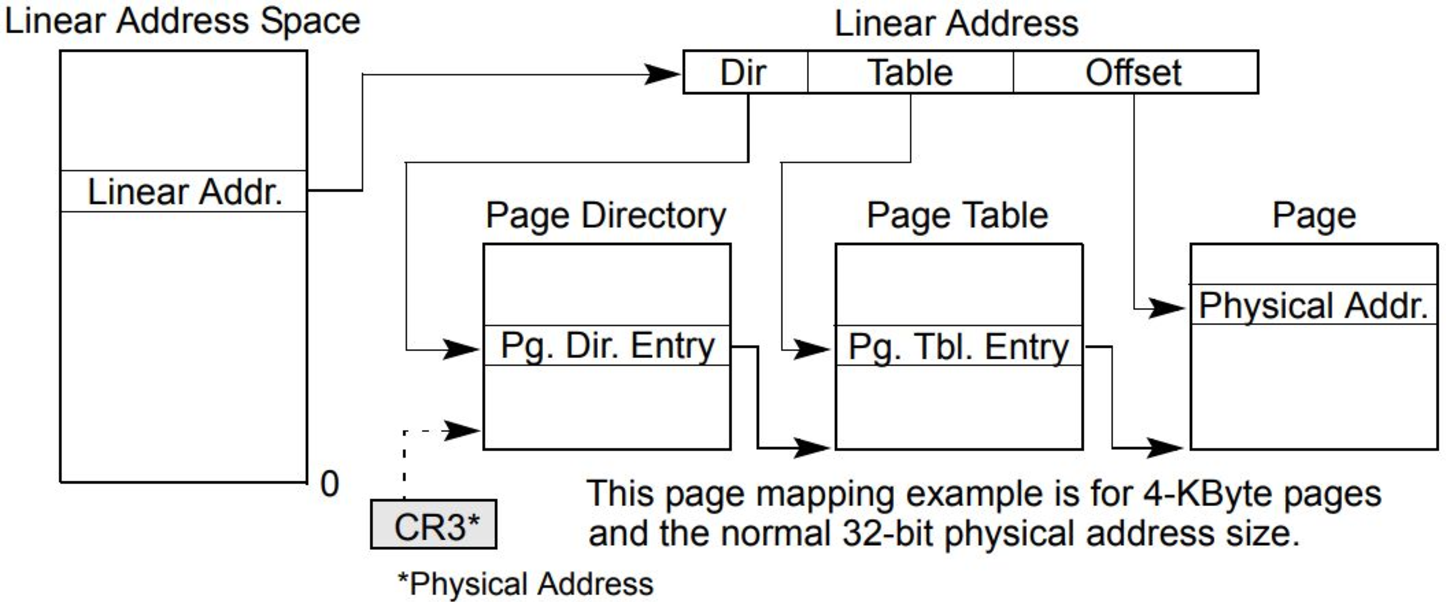
\includegraphics[width=0.47\textwidth]{figures/pagetable}
  \centering
  \caption{Linear-Address Translation to a 4-KBbyte Page using 32-Bit Paging~\cite{guide2011intel}}
  \label{fig:pagetable}
\end{figure}

\textbf{\textit{Translation Lookaside Buffer.}} As mentioned above, page table walking is a lengthy process. A full walk needs to access two pages (\texttt{PD} page and \texttt{PTE} page). If any of the two pages are not present in the memory (\texttt{PDE} or \texttt{PTE} invalid), it further triggers a page fault to bring the absent page back.

A \texttt{Translation Lookaside Buffer (TLB)} is a memory cache used to reduce the time for the processor to access a virtual memory address. It is part of \texttt{MMU}. A \texttt{TLB} has a fixed number of slots that stores the recent translations of virtual memory to physical memory and permission bits.  A \texttt{TLB} may reside between the processor and the processor cache or between the processor cache and the main memory. If valid \texttt{TLB} entry exists, the corresponded \texttt{PTE} is ignored. The system kernel is responsible for the consistency between \texttt{TLB} and page table.



\textbf{\textit{Interrupt Descriptor Table.}} The \texttt{Interrupt Descriptor Table (IDT)} is a data structure used on the x86 architecture to implement an interrupt vector table. The processor uses the \texttt{IDT} to determine the correct response to interrupts and exceptions. \texttt{IDTR} is the register on each processor to store the address of the \texttt{IDT}.

\textbf{\textit{Interrupts and Exceptions.}} The fundamental difference in microarchitecture between interrupt and exception is as follows.  An interrupt is an asynchronous event that is typically triggered by an I/O device. An exception is a synchronous event generated when the processor detects one or more predefined conditions while executing an instruction. However, one thing in common is that their handlers are all in the \texttt{IDT}, which makes them easy to confuse.

Furthermore, exceptions are classified as \textbf{faults}, \textbf{traps}, and \textbf{aborts} depending on the way they are reported and whether the instruction that caused the exception can be restarted without loss of program or task continuity. Aborts are not recoverable. They are used to report severe errors, such as hardware errors and inconsistent or illegal values in system tables. Faults and traps are recoverable, and the main difference between them is that when recovers from faults, the return address is the faulting instruction. On the other side, the trap's return address points to the instruction to be executed after the trapping instruction. In our case, the \texttt{SMAP} exception is a fault and handled through the page fault handler.

The \texttt{IDT} has 256 entries. Entry 0-31 are for exceptions except the entry 2 is for \texttt{Non-Maskable external Interrupt (NMI)}. The rest are for external interrupt from \texttt{INTR} pin or \texttt{INT n} instruction. However, \texttt{INT n} also known as a software interrupt. It is essentially an exception with "interrupt" in its name, and its vector located with other external hardware interrupt vectors. Fun.



\textbf{\textit{Trap Frame.}} It is the data structure pushed to the stack by the processor. It contains registers of the current thread when an interrupt or exception occurs. Each trap frame stores only a subset of the registers depending on scenarios, namely, the \texttt{SS:ESP} is pushed base on if there is a change in \texttt{Current Privilege Level (CPL)} of the \texttt{CS} register.  In the context of a page fault, \texttt{ErrorCode}, \texttt{CS:EIP}, \texttt{EFLAGS}, and \texttt{SS:ESP} are pushed into the kernel stack.



\textbf{\textit{Gate.}} Code modules in lower privilege segments can only access modules operating at higher privilege segments through a tightly controlled and protected interface called a \textbf{gate}.  There are four types of gate, namely, \textbf{task gate}, \textbf{trap gate}, \textbf{interrupt gate}, and \textbf{call gate}. Fully describe and distinguish them is out of the paper's scope. The project only involves the interrupt gate.

The vectors in the IDT go through either the interrupt gate or trap gate. The difference between them is as follows. If the interrupt or exception handler is called through an interrupt gate, the processor clears the \texttt{interrupt enable flag (IF)} in the \texttt{EFLAGS} register to prevent subsequent interrupts from interfering with the execution of the handler.  When the processor invokes a handler through a trap gate, it does not change the IF flag. Having \texttt{EFLAGS.IF} set is a requirement to control stack depth, which also involves what type of interrupt controller installed in the system. We observed that the processor invokes the page fault handler through an interrupt gate. We think the reason for that is as follows. The processor loads the \texttt{CR2} register with the 32-bit virtual address that generated the exception. Another page fault can potentially occur during the execution of the page fault handler. Hence the page fault handler should save the contents of the \texttt{CR2} before a second page fault can occur because the processor update \texttt{CR2} whenever a page fault is detected.

\textbf{\textit{CS Segment and Current Privilege Level}} \texttt{CS} segment register cannot be set directly through instruction \texttt{mov}, unlike other segment registers,  but only through a trap or interrupt gate. The system's current privilege level depends on the Current Privilege Level (CPL) field in the \texttt{CS} segment, which is maintained by the processor. This 2-bit CPL field in the code segment register is always equal to the processor's current privilege level. When getting the \texttt{CS} image from the trap frame of a page fault context, it provides us the ground truth of what privilege of the code when the \texttt{SMAP} exception happens, so that we do not make the decision based on the apparent value of \texttt{EIP}. To fully explain the privilege transition mechanism is out of the paper's scope.

\textbf{\textit{Inter-processor Interrupt.}}  It is an interrupt controller mechanism to interrupt another processor or group of processors on the system bus. They are used for software self-interrupts, interrupt forwarding, or preemptive scheduling. In \name, we use \texttt{IPI} to flush \texttt{TLB} cache on all the processors.

\textbf{\textit{Local APIC.}} Intel's Advanced Programmable Interrupt Controller (APIC) is a family of interrupt controllers. It is more advanced than Intel's 8259 Programmable Interrupt Controller (PIC). Nowadays, SMP systems with multiple processors utilize APIC. The APIC is a split architecture design, with a local APIC usually integrated into the processor and an optional I/O APIC on a system bus. The local APIC performs two primary functions for the processor:
It receives interrupts from the processor's interrupt pins, internal sources, and an external I/O APIC. It sends these to the processor core for handling.
It sends and receives IPI messages to and from other logical processors on the system bus in multiple-processor systems.
The external I/O APIC is part of Intel's system chipset. It is responsible for receiving interrupts generated by system hardware and I/O devices and forwarding them to the local APIC as interrupt messages. A processor can generate IPIs by programming the interrupt command register (ICR) in its local APIC. Writing to the ICR generates an IPI message on the system bus or the APIC bus. When the target processor receives an IPI message, its local APIC handles the message automatically using information included in the message such as vector number and trigger mode. The IPI mechanism sends interrupts for a specific vector number, and special-purpose interrupts to processors on the system bus. Local APIC registers are memory-mapped to a 4-KByte region of the processor's physical address space with an initial starting address of EFF00000H. The software interacts with the local APIC by reading and writing its registers. It also can change the initial mapping to a different 4-KByte region for all the local APICs. The presence of a local APIC can be detected using the CPUID instruction. Execute CPUID with source operand of 1 in the EAX register, then bit 9 of returned feature flags in EDX register indicate a local APIC.


\begin{figure}[th]
  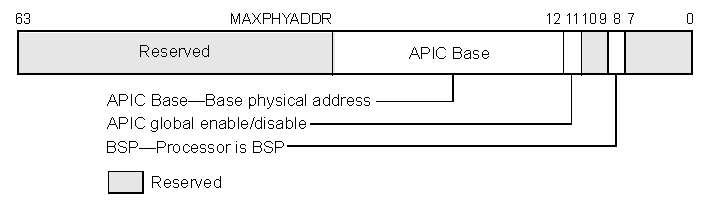
\includegraphics[width=0.40\textwidth]{figures/ia32apicbase}
  \centering
  \caption{\texttt{IA32\_APIC\_BASE} MSR}
  \label{fig:ia32apicbase}
\end{figure}

There is only one MSR associated with local APIC, \texttt{IA32\_APIC\_BASE}. As shown in~\autoref{fig:ia32apicbase}, the BSP flag indicates if the processor is the bootstrap processor (BSP); ``APIC global enable/disable'' enables/disables the APIC; APIC base specifies the base address of the APIC registers. This 24-bit value needs to be extended by 12 bits at the low end to form the base address. As formerly mentioned, this value by default is 0xFEE00000.

The primary local APIC facility for issuing IPIs is the interrupt command register (ICR), as shown in~\autoref{fig:icr}. It is a 64-bit local APIC register that allows the operating system to specify and send IPIs to processors in the system.


\begin{figure}[th]
  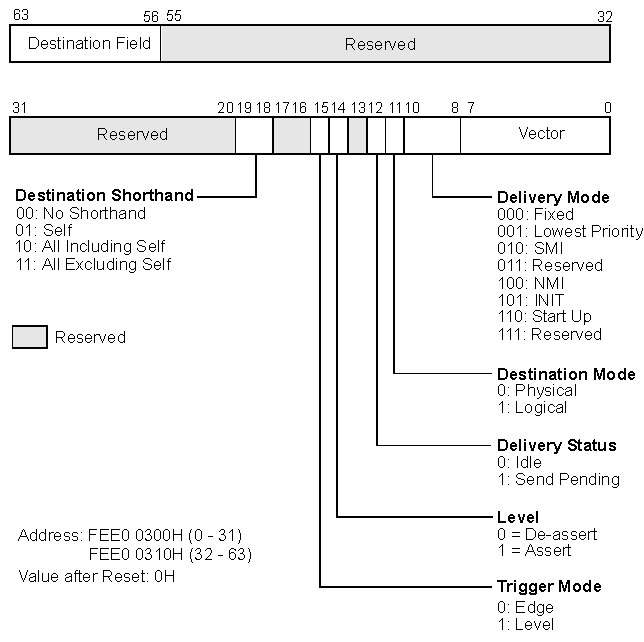
\includegraphics[width=0.40\textwidth]{figures/icr}
  \centering
  \caption{Interrupt Command Register (ICR)}
  \label{fig:icr}
\end{figure}

